\documentclass{standalone}
\usepackage{amsmath}
\usepackage[dvipsnames]{xcolor}
\usepackage{tikz} 
\usetikzlibrary{arrows, decorations.markings,decorations.pathreplacing,angles,quotes}
\usepackage{microtype}
\usepackage{fourier}

\definecolor{nblue}{RGB}{31, 119, 180}

\begin{document}


\begin{tikzpicture}
% include your tikz code here
   		\node[anchor=south west,inner sep=0] (Bild) at (0,0) {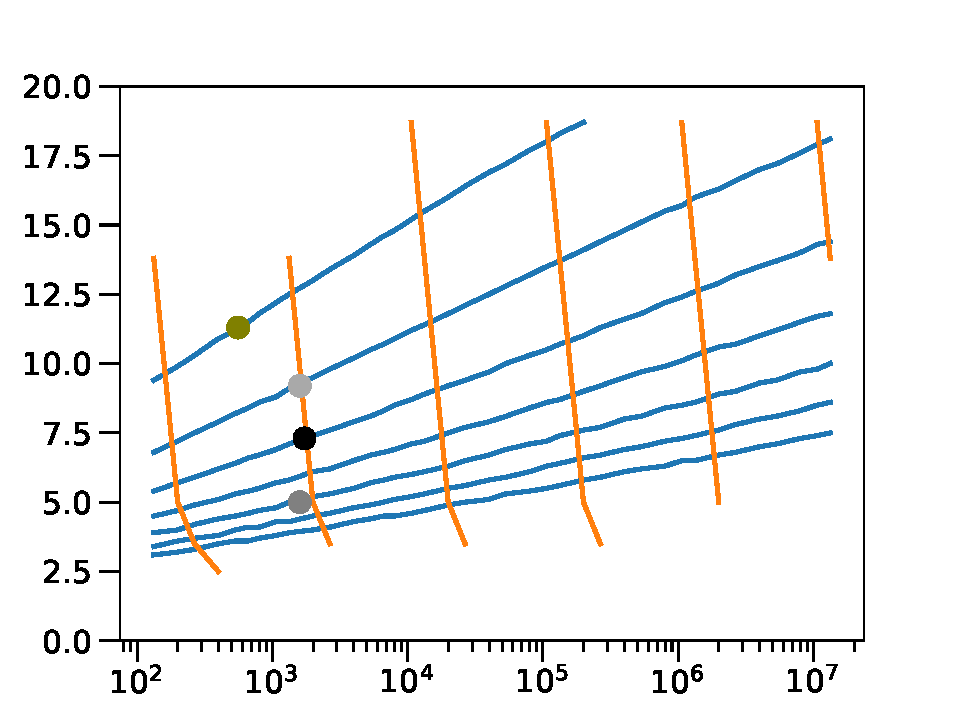
\includegraphics[scale=0.39]{fig1b_blank.pdf}};
   		\begin{scope}[x=(Bild.south east),y=(Bild.north west)]
        	\draw (0.5,-0.035) node {proportion of susceptible target cells};
        	\draw (-0.02,0.5) node [] {$R_0$};
        	
        	\draw[orange] (0.175,0.68) node {\tiny $10^6$};
        	\draw[orange] (0.36,0.82) node {\tiny $10^7$};
        	\draw[orange] (0.54,0.82) node {\tiny $10^8$};
        	\draw[orange] (0.71,0.82) node {\tiny $10^9$};
        	\draw[orange] (0.81,0.825) node {\tiny $10^{10}$};
        
        	\draw[nblue] (0.95,0.4) node {\tiny 9 days};
        	\draw[nblue] (0.95,0.44) node {\tiny 8 days};
        	\draw[nblue] (0.95,0.49) node {\tiny 7 days};
        	\draw[nblue] (0.95,0.56) node {\tiny 6 days};
        	\draw[nblue] (0.95,0.66) node {\tiny 5 days};
        	\draw[nblue] (0.95,0.8) node {\tiny 4 days};

			\fill[black] (0.6,0.25) circle (.07cm);
			\draw (0.6,0.25) node[right= 2pt] {\tiny Young et al. (2020)}; 
			\fill[lightgray,opacity=0.5] (0.6,0.2) circle (.07cm);   
			\draw (0.6,0.2) node[right= 2pt] {\tiny W{\"o}lfel et al. (2020)}; 			
			\fill[gray] (0.6,0.15) circle (.07cm);             	
        	\draw (0.6,0.15) node[right= 2pt] {\tiny France (unpublished)}; 
   		\end{scope}
\end{tikzpicture}

\end{document}